\section{Flag \& Ball Interaction} \label{flag-interaction}
This section codifies the rules for how the flags and the ball are interacted with.

Flags and balls are picked up automatically when a player enters their hex.

\subsection{The Flag}
The flag is present in each of the teams' capture zones.
The flag can be thrown (see \secref{throwing}) based on a player's \throw{} score (see \secref{the-team}).

\begin{table}[!ht]
    \centering
\begin{tabular}{r|l}
    \textbf{Point Value} & 1 \\
    \textbf{Movement Penalty} & $None$ \\
    \textbf{Can be Thrown?} & Yes \\
    \textbf{Special Note} & Capturing the flag doesn't immediately award points. \\
\end{tabular} 
    \caption{flag Stats}
    \label{tab:flag}
\end{table}
The thrown flag can be caught by an opposing player.
To do this, the pass must intersect the opposing player's reach.
The flag is successfully caught if the opposing player succeeds a \textit{Catch} check (see Section~\ref{sec:catching}).

Every opposing player whose reach it intersects gets an attempt at catching the throw.

\subsection{The Ball}
The Ball is a special heavy object that resides in the middle of the playing field.
The Ball is impractically heavy, and thus impedes movement, and cannot be thrown or sprinted with.
However, it can be handed off (see \secref{handing-off})

\begin{table}[!ht]
    \centering
\begin{tabular}{r|l}
    \textbf{Point Value} & $1$ \\
    \textbf{Movement Penalty} & $Mov/2$, rounded down \\
    \textbf{Can be Thrown?} & No, but can be handed off \\
    \textbf{Special Note} & Ends an Act the moment it's captured.\\
\end{tabular}
    \caption{Heavy Stats}
    \label{tab:heavy}
\end{table}
You only receive points for flags in your capture zone at the end of an Act; thus you only score when The Ball is captured.

\begin{note}
    You score for your own flag, should it still rest in your capture zone at the end of an Act.
\end{note}

\subsection{Throwing}\label{throwing}
To throw a flag, you must designate a target hex.
Then, depending on the distance, the throw is either \textit{sure} or \textit{unsure}.

\begin{description}
    \item[Sure Throw] Distance thrown $\leq Thr$. Guaranteed to hit target.
    \item[Unsure Throw] Distance thrown between $Thr$ and $2\times Thr$. Flag lands within scatter zone (see Section~\ref{scattering}).
\end{description}

Remember, flags are automatically picked up by a player where it lands. You can exploit this fact to chain throws.

\begin{note}
    Throwing can happen in any direction, not just along the six cardinals (see figure \ref{fig:line-throw}).
\end{note}

\begin{figure}
    \centering
    \includegraphics{graphics/throwing-cropped.png}
    \caption{A straight line approximated.}
    \label{fig:line-throw}
\end{figure}

\subsubsection{Attacking With the Flag} 
A flag may also be thrown with malicious intent.
When doing so, a target is designated as normal, but on a hit, the target is downed instead of catching the flag.
The flag remains in the downed target's hex, and can be picked up by other players.

On a miss, the flag scatters.

\begin{note}
    Missed attack throws can still be caught if it scatters into a player's hex.
\end{note}

\subsection{Getting Attacked}
If any attack downs a player holding the ball or flag, it scatters the object as if it had been thrown.

\subsection{Dropping the Flag}
You can drop a flag as part of a regular move action.
You simply leave it where it is and continue moving.

\subsection{Out of Bounds}
If a player throws a flag out of bounds it is out of play for the rest of the Act.

Should the ball fall out of bounds, it ends the Act and nobody is awarded any points.

\subsection{Scattering}\label{scattering}
To scatter a ball or flag, draw a card from the top of the deck (or cheat destiny).
The scattered object will then land on any of the hexes indicated by the scattering diagram\figref{fig:scatter-alternative}.

\begin{note}
    Drawing a Joker lets the player choose which hex the flag lands in.
\end{note}

\begin{figure}
    \centering
    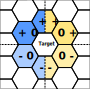
\includegraphics{graphics/scatter.png}
    \caption{Scattering.}
    \label{fig:scatter-alternative}
\end{figure}